\documentclass[10pt,a4paper]{article}
\usepackage[utf8]{inputenc}
\usepackage[top=2cm,bottom=2cm,left=2cm,right=2cm]{geometry}
\usepackage{amsmath}
\usepackage{amssymb}
\usepackage{array}
\usepackage{tikz}
\usetikzlibrary{arrows.meta,calc,patterns,positioning}
\usepackage{pgfplots}
\pgfplotsset{compat=1.18}
\usepackage[dvipsnames,svgnames]{xcolor}
\usepackage{hyperref}

% Anchor persamaan unik meski nomor di-reset per soal.
\newcounter{eqblock}
\newcommand{\reseteq}{%
  \stepcounter{eqblock}%
  \setcounter{equation}{0}%
  \renewcommand{\theHequation}{\arabic{eqblock}.\arabic{equation}}%
}

\pgfplotsset{
  grafik/.style={
    axis lines=middle,
    xlabel={$x$}, ylabel={$y$},
    width=7.5cm, height=6cm,
    grid=major, grid style={gray!25},
    tick label style={font=\scriptsize},
    every axis x label/.style={at={(ticklabel* cs:1)},anchor=west},
    every axis y label/.style={at={(ticklabel* cs:1)},anchor=south},
    title style={yshift=2ex},
  },
}

\title{Tugas Minggu 6 : Turunan}
\author{Matematika untuk Sistem Informasi}
\date{}

\begin{document}

\maketitle

\begin{enumerate}

%===========================================================
\item Tentukan turunan pertama dari $f(x) = x^2 + 2x + 1$ menggunakan definisi.

\textbf{Jawab:}
\begin{itemize}
\item \textbf{Langkah 1: Tulis Definisi dan Hitung $f(x + h) - f(x)$}

$\displaystyle f'(x) = \lim_{h \to 0} \frac{f(x + h) - f(x)}{h}$, dengan
\reseteq
\begin{align}
f(x + h) &= (x + h)^2 + 2(x + h) + 1 = x^2 + 2xh + h^2 + 2x + 2h + 1 \\
f(x + h) - f(x) &= (x^2 + 2xh + h^2 + 2x + 2h + 1) - (x^2 + 2x + 1) = 2xh + h^2 + 2h
\end{align}

\item \textbf{Langkah 2: Bagi dengan $h$ dan Ambil Limit}

\reseteq
\begin{align}
f'(x) &= \lim_{h \to 0} \frac{2xh + h^2 + 2h}{h} = \lim_{h \to 0} \frac{h(2x + h + 2)}{h} \quad \text{(Faktorkan $h$)} \\
&= \lim_{h \to 0} (2x + h + 2) = 2x + 2 \quad \text{(Coret $h \neq 0$, lalu substitusi $h = 0$)}
\end{align}
Jadi $f'(x) = 2x + 2$.
% final: f'(x) = 2x + 2
\end{itemize}

%===========================================================
\item Diketahui
\[
f(x) =
\begin{cases}
  x^2 - 1, & x < 3 \\
  6x - 10, & x \geq 3
\end{cases}
\]
Periksa apakah $f$ diferensiabel di $x = 3$. Kemudian tentukan nilai $f'(3)$ jika ada.

\textbf{Jawab:}
\begin{itemize}
\item \textbf{Langkah 1: Hitung $f(3)$}

\reseteq
\begin{align}
f(3) &= 6(3) - 10 = 8 \quad \text{(Aturan untuk $x \geq 3$)}
\end{align}

\item \textbf{Langkah 2: Periksa Kekontinuan di $x = 3$}

Fungsi yang tidak kontinu pasti tidak diferensiabel, sehingga kekontinuan diperiksa lebih dahulu.
\reseteq
\begin{align}
\lim_{x \to 3^-} f(x) &= \lim_{x \to 3^-} (x^2 - 1) = 9 - 1 = 8 \quad \text{(Aturan untuk $x < 3$)} \\
\lim_{x \to 3^+} f(x) &= \lim_{x \to 3^+} (6x - 10) = 18 - 10 = 8 \quad \text{(Aturan untuk $x > 3$)}
\end{align}
Karena $\lim_{x \to 3^-} f(x) = \lim_{x \to 3^+} f(x) = f(3) = 8$, maka $f$ kontinu di $x = 3$.

\item \textbf{Langkah 3: Hitung Turunan Kiri dan Turunan Kanan}

\reseteq
\begin{align}
f'_-(3) &= \lim_{x \to 3^-} \frac{(x^2 - 1) - 8}{x - 3} = \lim_{x \to 3^-} \frac{(x - 3)(x + 3)}{x - 3} = \lim_{x \to 3^-} (x + 3) = 6 \\
f'_+(3) &= \lim_{x \to 3^+} \frac{(6x - 10) - 8}{x - 3} = \lim_{x \to 3^+} \frac{6(x - 3)}{x - 3} = 6
\end{align}

\item \textbf{Langkah 4: Kesimpulan}

Karena $f'_-(3) = f'_+(3) = 6$, maka $f$ \textbf{diferensiabel} di $x = 3$ dan $f'(3) = 6$.
% final: f'(3) = 6
\end{itemize}

%===========================================================
\item Diketahui
\[
f(x) =
\begin{cases}
  -x^2 + 1, & x \leq 1 \\
  x - 1, & x > 1
\end{cases}
\]
Periksa apakah $f$ diferensiabel di $x = 1$. Kemudian tentukan nilai $f'(1)$ jika ada.

\textbf{Jawab:}
\begin{itemize}
\item \textbf{Langkah 1: Hitung $f(1)$}

\reseteq
\begin{align}
f(1) &= -(1)^2 + 1 = 0 \quad \text{(Aturan untuk $x \leq 1$)}
\end{align}

\item \textbf{Langkah 2: Periksa Kekontinuan di $x = 1$}

\reseteq
\begin{align}
\lim_{x \to 1^-} f(x) &= \lim_{x \to 1^-} (-x^2 + 1) = -1 + 1 = 0 \quad \text{(Aturan untuk $x < 1$)} \\
\lim_{x \to 1^+} f(x) &= \lim_{x \to 1^+} (x - 1) = 1 - 1 = 0 \quad \text{(Aturan untuk $x > 1$)}
\end{align}
Karena $\lim_{x \to 1^-} f(x) = \lim_{x \to 1^+} f(x) = f(1) = 0$, maka $f$ kontinu di $x = 1$.

\item \textbf{Langkah 3: Hitung Turunan Kiri dan Turunan Kanan}

\reseteq
\begin{align}
f'_-(1) &= \lim_{x \to 1^-} \frac{(-x^2 + 1) - 0}{x - 1} = \lim_{x \to 1^-} \frac{-(x - 1)(x + 1)}{x - 1} = \lim_{x \to 1^-} \bigl(-(x + 1)\bigr) = -2 \\
f'_+(1) &= \lim_{x \to 1^+} \frac{(x - 1) - 0}{x - 1} = \lim_{x \to 1^+} 1 = 1
\end{align}

\item \textbf{Langkah 4: Kesimpulan}

Karena $f'_-(1) = -2 \neq 1 = f'_+(1)$, maka $f$ \textbf{tidak diferensiabel} di $x = 1$ dan $f'(1)$ tidak ada.
Walaupun $f$ kontinu di $x = 1$, grafiknya membentuk sudut (patah) di titik $(1, 0)$:

\begin{center}
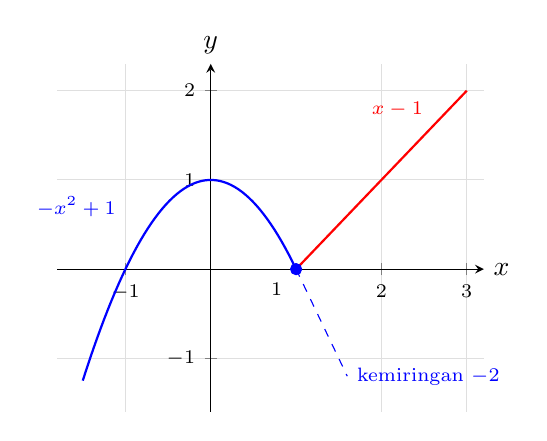
\begin{tikzpicture}
\begin{axis}[grafik, width=7cm, height=6cm, clip=false, xmin=-1.8, xmax=3.2, ymin=-1.6, ymax=2.3, xtick={-1,2,3}, ytick={-1,1,2}]
  \addplot[domain=-1.5:1, samples=60, thick, blue] {-x^2 + 1};
  \addplot[domain=1:3, thick, Red] {x - 1};
  \addplot[domain=1:1.6, dashed, blue] {-2*(x - 1)};
  \filldraw[blue] (axis cs:1,0) circle (2pt);
  \node[font=\scriptsize, anchor=north east] at (axis cs:0.95,-0.05) {$1$};
  \node[font=\scriptsize, blue, anchor=east] at (axis cs:-1,0.7) {$-x^2 + 1$};
  \node[font=\scriptsize, Red, anchor=south east] at (axis cs:2.6,1.6) {$x - 1$};
  \node[font=\scriptsize, blue, anchor=west] at (axis cs:1.6,-1.2) {kemiringan $-2$};
\end{axis}
\end{tikzpicture}
\end{center}
Garis putus-putus adalah arah garis singgung dari kiri (kemiringan $-2$), sedangkan dari kanan kemiringannya $1$.
% final: f'(1) \text{ tidak ada}
\end{itemize}

%===========================================================
\item Tentukan turunan pertama dari fungsi berikut:
\begin{enumerate}

%-----------------------------------------------------------
\item $f(x) = (x^2 + 1)(x^3 - 3x + 1)$

\textbf{Jawab:}
\begin{itemize}
\item \textbf{Langkah 1: Aturan Hasil Kali}

Misalkan $u = x^2 + 1$ ($u' = 2x$) dan $v = x^3 - 3x + 1$ ($v' = 3x^2 - 3$).
\reseteq
\begin{align}
f'(x) &= u'v + uv' = 2x(x^3 - 3x + 1) + (x^2 + 1)(3x^2 - 3) \\
&= (2x^4 - 6x^2 + 2x) + (3x^4 - 3x^2 + 3x^2 - 3) \quad \text{(Jabarkan)} \\
&= 5x^4 - 6x^2 + 2x - 3
\end{align}
% final: f'(x) = 5x^4 - 6x^2 + 2x - 3
\end{itemize}

%-----------------------------------------------------------
\item $f(x) = \dfrac{x - 3}{1 - x^2}$

\textbf{Jawab:}
\begin{itemize}
\item \textbf{Langkah 1: Aturan Hasil Bagi}

Misalkan $u = x - 3$ ($u' = 1$) dan $v = 1 - x^2$ ($v' = -2x$).
\reseteq
\begin{align}
f'(x) &= \frac{u'v - uv'}{v^2} = \frac{1 \cdot (1 - x^2) - (x - 3)(-2x)}{(1 - x^2)^2} \\
&= \frac{1 - x^2 + 2x^2 - 6x}{(1 - x^2)^2} = \frac{x^2 - 6x + 1}{(1 - x^2)^2}
\end{align}
% final: f'(x) = \frac{x^2 - 6x + 1}{(1 - x^2)^2}
\end{itemize}

%-----------------------------------------------------------
\item $f(x) = x^2 \sin x$

\textbf{Jawab:}
\begin{itemize}
\item \textbf{Langkah 1: Aturan Hasil Kali}

Misalkan $u = x^2$ ($u' = 2x$) dan $v = \sin x$ ($v' = \cos x$).
\reseteq
\begin{align}
f'(x) &= 2x\sin x + x^2\cos x = x(2\sin x + x\cos x)
\end{align}
% final: f'(x) = 2x\sin x + x^2\cos x
\end{itemize}

%-----------------------------------------------------------
\item $f(x) = \dfrac{1 + \sin x}{\cos x}$

\textbf{Jawab:}
\begin{itemize}
\item \textbf{Langkah 1: Aturan Hasil Bagi}

Misalkan $u = 1 + \sin x$ ($u' = \cos x$) dan $v = \cos x$ ($v' = -\sin x$).
\reseteq
\begin{align}
f'(x) &= \frac{\cos x \cdot \cos x - (1 + \sin x)(-\sin x)}{\cos^2 x} = \frac{\cos^2 x + \sin x + \sin^2 x}{\cos^2 x} \\
&= \frac{1 + \sin x}{\cos^2 x} \quad \text{(Identitas $\sin^2 x + \cos^2 x = 1$)}
\end{align}
% final: f'(x) = \frac{1 + \sin x}{\cos^2 x}
\end{itemize}

%-----------------------------------------------------------
\item $f(x) = (2x^2 - 4x + 1)^{60}$

\textbf{Jawab:}
\begin{itemize}
\item \textbf{Langkah 1: Aturan Rantai}

Misalkan $u = 2x^2 - 4x + 1$, sehingga $f = u^{60}$ dan $\frac{du}{dx} = 4x - 4 = 4(x - 1)$.
\reseteq
\begin{align}
f'(x) &= 60u^{59} \cdot \frac{du}{dx} = 60(2x^2 - 4x + 1)^{59} \cdot 4(x - 1) \\
&= 240(x - 1)(2x^2 - 4x + 1)^{59}
\end{align}
% final: f'(x) = 240(x - 1)(2x^2 - 4x + 1)^{59}
\end{itemize}

%-----------------------------------------------------------
\item $f(x) = \cos^4(4x^2 - x)$

\textbf{Jawab:}
\begin{itemize}
\item \textbf{Langkah 1: Aturan Rantai Tiga Lapis}

$f(x) = \bigl[\cos(4x^2 - x)\bigr]^4$. Misalkan $v = 4x^2 - x$, $u = \cos v$, dan $f = u^4$.
\reseteq
\begin{align}
f'(x) &= \frac{df}{du} \cdot \frac{du}{dv} \cdot \frac{dv}{dx} = 4u^3 \cdot (-\sin v) \cdot (8x - 1) \\
&= -4(8x - 1)\cos^3(4x^2 - x)\sin(4x^2 - x)
\end{align}
% final: f'(x) = -4(8x - 1)\cos^3(4x^2 - x)\sin(4x^2 - x)
\end{itemize}

\end{enumerate}

%===========================================================
\item Carilah turunan kedua dari fungsi berikut:
\begin{enumerate}

%-----------------------------------------------------------
\item $f(x) = \sin(2x - 1)$

\textbf{Jawab:}
\begin{itemize}
\item \textbf{Langkah 1: Turunan Pertama}

\reseteq
\begin{align}
f'(x) &= \cos(2x - 1) \cdot 2 = 2\cos(2x - 1) \quad \text{(Aturan rantai, $u = 2x - 1$)}
\end{align}

\item \textbf{Langkah 2: Turunan Kedua}

\reseteq
\begin{align}
f''(x) &= 2\bigl(-\sin(2x - 1)\bigr) \cdot 2 = -4\sin(2x - 1)
\end{align}
% final: f''(x) = -4\sin(2x - 1)
\end{itemize}

%-----------------------------------------------------------
\item $f(x) = (2x - 3)^4$

\textbf{Jawab:}
\begin{itemize}
\item \textbf{Langkah 1: Turunan Pertama}

\reseteq
\begin{align}
f'(x) &= 4(2x - 3)^3 \cdot 2 = 8(2x - 3)^3 \quad \text{(Aturan rantai, $u = 2x - 3$)}
\end{align}

\item \textbf{Langkah 2: Turunan Kedua}

\reseteq
\begin{align}
f''(x) &= 8 \cdot 3(2x - 3)^2 \cdot 2 = 48(2x - 3)^2
\end{align}
% final: f''(x) = 48(2x - 3)^2
\end{itemize}

\end{enumerate}

%===========================================================
\item Tentukan persamaan garis singgung dan garis normal fungsi $y = (2x + 1)^3$ di titik $(0, 1)$.

\textbf{Jawab:}
\begin{itemize}
\item \textbf{Langkah 1: Pastikan Titik pada Kurva}

$y(0) = (2 \cdot 0 + 1)^3 = 1$, jadi titik $(0, 1)$ terletak pada kurva.

\item \textbf{Langkah 2: Hitung Kemiringan Garis Singgung}

\reseteq
\begin{align}
y' &= 3(2x + 1)^2 \cdot 2 = 6(2x + 1)^2 \quad \text{(Aturan rantai)} \\
m &= y'(0) = 6(1)^2 = 6
\end{align}

\item \textbf{Langkah 3: Garis Singgung}

\reseteq
\begin{align}
y - 1 &= 6(x - 0) \\
y &= 6x + 1
\end{align}

\item \textbf{Langkah 4: Garis Normal}

Kemiringan garis normal $m_n = -\frac{1}{m} = -\frac{1}{6}$:
\reseteq
\begin{align}
y - 1 &= -\frac{1}{6}(x - 0) \\
y &= -\frac{1}{6}x + 1
\end{align}

\item \textbf{Langkah 5: Gambar}

\begin{center}
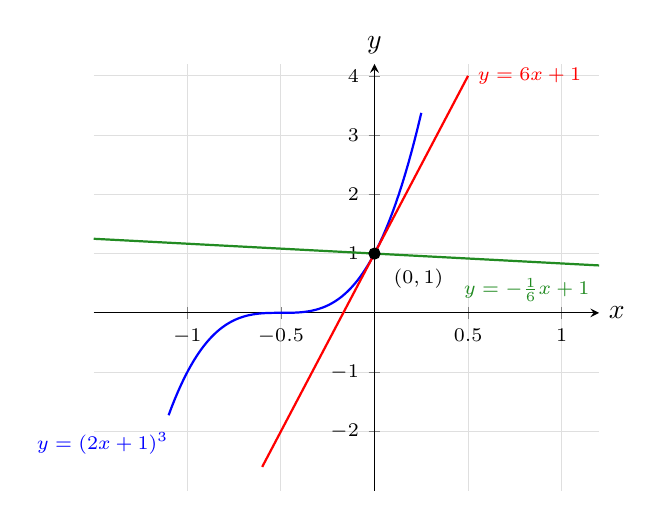
\begin{tikzpicture}
\begin{axis}[grafik, width=8cm, height=7cm, clip=false, xmin=-1.5, xmax=1.2, ymin=-3, ymax=4.2, xtick={-1,-0.5,0.5,1}, ytick={-2,-1,1,2,3,4}]
  \addplot[domain=-1.1:0.25, samples=80, thick, blue] {(2*x + 1)^3};
  \addplot[domain=-0.6:0.5, thick, Red] {6*x + 1};
  \addplot[domain=-1.5:1.2, thick, ForestGreen] {-x/6 + 1};
  \filldraw[black] (axis cs:0,1) circle (2pt);
  \node[font=\scriptsize, anchor=north west] at (axis cs:0.05,0.9) {$(0,1)$};
  \node[font=\scriptsize, blue, anchor=east] at (axis cs:-1.05,-2.2) {$y = (2x + 1)^3$};
  \node[font=\scriptsize, Red, anchor=west] at (axis cs:0.5,4) {$y = 6x + 1$};
  \node[font=\scriptsize, ForestGreen, anchor=north east] at (axis cs:1.2,0.75) {$y = -\frac{1}{6}x + 1$};
\end{axis}
\end{tikzpicture}
\end{center}
Skala sumbu $x$ dan $y$ berbeda, sehingga sudut siku-siku antara kedua garis tidak tampak tegak lurus pada gambar.
% final: y = 6x + 1
% final: y = -\frac{1}{6}x + 1
\end{itemize}

\end{enumerate}

\end{document}
